\chapter{Présentation de l'organisme d'acceuil Sirius Digital}
\clearpage
\section{Historique de Sirius Digital}

\subsection{Historique}

Fondée en 2022 par OURO BODI, Sirius Digital est une startup informatique basée à Lomé, dans le quartier de Kegué, en face du complexe scolaire Dino Golo. Dès ses débuts, l’entreprise s’est donnée pour mission de concevoir des solutions numériques innovantes répondant aux défis technologiques des entreprises, qu'elles soient petites ou grandes.

Face à l'\ac{essor} rapide des nouvelles technologies et à l’évolution croissante des besoins dans tous les secteurs, Sirius Digital s’impose progressivement comme un acteur clé dans le développement d’applications web et mobiles. Grâce à une approche axée sur l’innovation et la qualité, la startup accompagne les entreprises dans leur transformation digitale, leur offrant des outils performants et adaptés à leurs réalités.

Aujourd’hui, Sirius Digital continue d’évoluer en mettant la technologie au service du développement, avec pour ambition de devenir une référence incontournable dans le domaine des solutions numériques en Afrique et au-delà.


\begin{itemize}
    \item \textbf{Adresse :} Kegué, Lomé-TOGO, 16BP:20
    \item \textbf{Téléphone :} (+228) 91 09 16 56 / 22 61 78 84
    \item \textbf{E-mail :} \href{mailto:siriusdigital@app-siriusdigital.com}{siriusdigital@app-siriusdigital.com}
    \item \textbf{Site web :} \href{https://app-siriusdigital.com}{app-siriusdigital.com}
\end{itemize}



\section{Les organes de SIRIUS DIGITAL}
\begin{center}
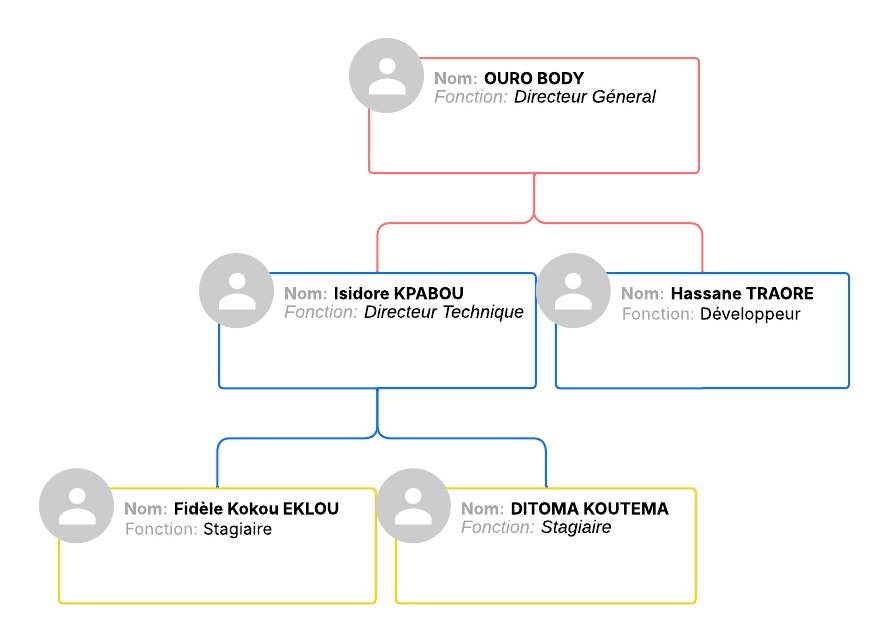
\includegraphics[scale=0.5]{images/logo/foc.png}
\end{center}




\clearpage